% JW-FD SPIE Proceedings manuscript (expanded, ~6 pages)
\documentclass[]{spie}

\usepackage{graphicx}
\usepackage{amsmath}
\usepackage{booktabs}
\usepackage{tikz}
\usetikzlibrary{positioning,arrows.meta,shapes.geometric}

\title{An end-to-end pipeline for multimodal solar flare forecasting dataset construction}

\author{Shao Mingfu\supit{a}, Lin Jiaben\supit{a}, Wang Hui\supit{a}, Tong Liyue\supit{a}, and Li Yuyang\supit{a}
\skiplinehalf
\supit{a}National Astronomical Observatories, Chinese Academy of Sciences, Beijing, China
}

\authorinfo{Correspondence: Shao Mingfu. E-mail: shaomf@bao.ac.cn}

\begin{document}
\maketitle

\begin{abstract}
Solar flares are primary drivers of space weather; forecasting eruption from photospheric magnetograms remains a central challenge for solar physics and operational services. Existing flare datasets often provide short temporal coverage, single-modality releases, rigid label systems, and risk cross-split leakage when samples from the same active region (AR) appear in both training and test partitions. We present \textbf{JW-FD} (JW Flare Dataset), a long-horizon multimodal benchmark built through a documented six-step automated pipeline. JW-FD links NOAA X-ray flare events to 600$\times$600~pixel SDO/HMI line-of-sight magnetogram crops tracked per NOAA AR, spanning 1~January~2011 through 31~December~2024 (14~years). The release comprises 2{,}687 independent ARs, 1{,}750{,}184 co-registered snapshots, and 2{,}687 per-AR evolution videos, exported as FITS, PNG, CSV, and MP4 modalities. Each CSV record binds 29 magnetic features, 35 configurable flare-label fields, and 2 metadata columns (66~dimensions total). Labels follow strict pre-eruption semantics over seven prediction horizons and four GOES thresholds. An 8:1:1 AR-level split prevents temporal leakage. The open-source pipeline is available at \texttt{https://github.com/Xiaoxuan-1/JW-FD}.
\end{abstract}

\keywords{solar flare forecasting, HMI magnetograms, multimodal dataset, space weather, active regions}

\section{INTRODUCTION}
\label{sec:intro}

Solar flares are among the most energetic manifestations of solar magnetic activity. Major flares (M/X-class on the GOES scale) can disrupt satellite operations, aviation communications, and power-grid infrastructure. Forecasting flare occurrence \emph{before} eruption from photospheric magnetograms is therefore a priority for both fundamental solar physics and operational space-weather services.\cite{Shao2025review,Toriumi2019,Leka2019}

Photospheric line-of-sight (LOS) magnetograms encode magnetic complexity---gradient concentrations, neutral-line topology, and flux imbalance---that precede many eruptive events.\cite{Boucheron2015,Bobra2014} Quantitative descriptors derived from magnetograms have long supported statistical and machine-learning (ML) flare-forecasting models. Recent work extends this paradigm to convolutional networks, vision transformers, and multimodal large language models (MLLMs) that consume both images and structured physical parameters.\cite{Shao2025jwflare} Such methods require corpora in which visual, tabular, and label modalities are co-registered in space and time, with evaluation protocols that prevent information leakage across training and test partitions.

Traditional flare datasets frequently exhibit four limitations: (1)~temporal coverage shorter than a full solar cycle; (2)~release of either images \emph{or} tabular parameters but not both at pixel-level alignment; (3)~fixed label definitions that do not support multiple forecast horizons or intensity thresholds; and (4)~sample-level splits that place different timestamps of the same AR in training and test sets, inflating performance through temporal autocorrelation.\cite{Bloomfield2012,Barnes2016}

\textbf{JW-FD} addresses these gaps with a reproducible six-step pipeline that ingests NOAA/USAF Solar Region Summary (SRS) reports, NOAA Events X-ray (XRA) flare lists, and SDO/HMI\cite{Scherrer2012,Pesnell2012} full-disk LOS magnetograms. Our contributions are:
\begin{enumerate}
\item A \textbf{14-year multimodal release} (2011--2024) covering solar cycles~24--25 with 1.75~million AR snapshots, enabling study of cycle-dependent flare statistics and rare X-class events.
\item A \textbf{documented, modular six-step pipeline} with multiprocessing support and configurable parameters (magnetic saturation threshold, forecast horizons, year range), supporting reproducible extension as new HMI data arrive.
\item \textbf{Configurable multi-horizon, multi-threshold labels} with strict pre-eruption semantics: positive labels only within the half-open interval $[\mathrm{Begin}-h,\,\mathrm{Begin})$, distinguishing forecasting from nowcasting.
\item An \textbf{8:1:1 AR-level train/validation/test split} that keeps all timestamps of one AR in a single partition, establishing a leakage-free benchmark for classical ML, deep vision models, and MLLMs.
\end{enumerate}

Section~\ref{sec:related} reviews related datasets and evaluation practices. Section~\ref{sec:overview} describes data sources and organization. Section~\ref{sec:pipeline} details the construction pipeline. Sections~\ref{sec:schema}--\ref{sec:alignment} define the record schema, labeling rules, and multimodal alignment. Section~\ref{sec:qc} covers quality assurance and the evaluation protocol. Section~\ref{sec:concl} concludes.

\section{RELATED WORK}
\label{sec:related}

Flare forecasting from photospheric magnetic fields has progressed from hand-crafted region parameters to automated feature extraction and ML classifiers.\cite{Boucheron2015,Bobra2014} Boucheron et al.\ extracted multivariate time series of gradient, neutral-line, wavelet, and flux features from magnetograms and demonstrated competitive flare prediction with support-vector machines.\cite{Boucheron2015} Operational and research forecasting systems have since incorporated Space-weather HMI Active Region Patch (SHARP) vector-field parameters and diverse ML architectures.\cite{Barnes2016,Leka2019}

Dataset construction for this field remains fragmented. Many releases provide either image sequences or tabular feature tables without guaranteed pixel-level correspondence. Temporal spans are often limited to a single solar cycle or a few years. Label definitions vary across studies: some treat any pre-flare magnetogram as positive, while operational forecasting requires explicit forecast horizons. Bloomfield et al.\ emphasized the need for standardized benchmarks and metrics;\cite{Bloomfield2012} Barnes et al.\ showed that evaluation design---including whether consecutive days from the same AR appear in both training and test sets---strongly affects reported skill scores.\cite{Barnes2016,Leka2019}

Recent MLLM-based approaches motivate multimodal corpora that bind magnetograms, physical descriptors, and flare metadata in a single index.\cite{Shao2025jwflare,Shao2025review} JW-FD is designed as infrastructure for such methods rather than as a model paper: it supplies aligned FITS/PNG/CSV/MP4 products, configurable labels, and a documented AR-level split.

\begin{table}[t]
\caption{Comparison of JW-FD with representative prior flare-forecasting datasets.}
\label{tab:comparison}
\centering
\small
\begin{tabular}{@{}p{2.6cm}p{3.8cm}p{3.8cm}@{}}
\toprule
Dimension & JW-FD & Typical prior datasets \\
\midrule
Temporal span & 14~yr (2011--2024) & $\sim$8~yr or less \\
Modalities & FITS + PNG + CSV + MP4 & Image \emph{or} parameters \\
Label flexibility & 7 horizons $\times$ 4 thresholds & Fixed horizon/class \\
Split protocol & 8:1:1 by AR & Often sample-level \\
Pipeline & Open six-step code & Ad hoc scripts \\
\bottomrule
\end{tabular}
\end{table}

Table~\ref{tab:comparison} summarizes JW-FD's positioning. By integrating long-horizon coverage, multimodal exports, flexible labels, and a leakage-aware split within one reproducible pipeline, JW-FD complements feature-based benchmarks such as Ref.~\citenum{Boucheron2015} and evaluation frameworks such as Refs.~\citenum{Bloomfield2012,Barnes2016}.

\section{DATA SOURCES AND DATASET OVERVIEW}
\label{sec:overview}

\subsection{Observational inputs}

JW-FD draws on three public data streams. \textbf{SDO/HMI}\cite{Scherrer2012,Pesnell2012} provides full-disk LOS magnetograms at 4096$\times$4096 pixels ($\sim$1.5$''$ per pixel) with a cadence of approximately 12~minutes. \textbf{NOAA/USAF Solar Region Summary (SRS)} reports list daily NOAA AR numbers and heliographic locations in a compact string format (e.g., N12W45).\cite{NOAA2024events} \textbf{NOAA Events} files record GOES soft X-ray (XRA) flare begin, maximum, and end times together with GOES class strings (C, M, or X followed by a numeric sub-class).

These sources span solar cycles~24 and the rising phase of cycle~25, capturing both quiet-Sun and active-Sun epochs and providing statistically meaningful samples of C-, M-, and X-class events.

\subsection{Dataset scale and modalities}

JW-FD is organized around NOAA active regions as the fundamental entity. Every snapshot---FITS crop, PNG frame, CSV row, and MP4 frame---is keyed by AR number and UTC timestamp derived from the original HMI filename.

\begin{table}[t]
\caption{JW-FD dataset summary.}
\label{tab:summary}
\centering
\small
\begin{tabular}{@{}ll@{}}
\toprule
Item & Value \\
\midrule
Temporal coverage & 2011-01-01 -- 2024-12-31 (14~yr) \\
Active regions & 2{,}687 independent NOAA ARs \\
Effective snapshots & 1{,}750{,}184 \\
Spatial resolution & 600$\times$600~pixels per crop \\
Modalities & FITS, PNG, CSV, MP4 (2{,}687 videos) \\
Standard split & 8:1:1 by AR (train / val / test) \\
Data sources & SDO/HMI LOS; NOAA SRS; NOAA Events (XRA) \\
\bottomrule
\end{tabular}
\end{table}

Table~\ref{tab:summary} lists the principal scale metrics. \textbf{FITS} files preserve magnetic field values in Gauss. \textbf{PNG} images apply configurable saturation and linear normalization to 8-bit grayscale for vision-model input. \textbf{CSV} files index every snapshot with 29 physics-based magnetic descriptors and 35 flare-label dimensions. \textbf{MP4} videos concatenate each AR's PNG sequence at 60~frames per second for temporal models.

\subsection{Storage organization}

Processed data follow a consistent directory hierarchy under a configurable output root (\texttt{OUTPUT\_PATH}):
\begin{verbatim}
fits_600/{ARnum}/AR{num}_{timestamp}.fits
png_600_Th{B_th}/{ARnum}/AR{num}_{timestamp}.png
solar_flare_dataset_{fits|png}_Lat{lat}_Lon{lon}_Th{B_th}.csv
movies_600_Th{B_th}/AR{num}_evolution.mp4
\end{verbatim}
The filename suffix encodes latitude/longitude filter bounds and magnetic threshold via \texttt{get\_output\_suffix()} in the pipeline configuration. Year filtering (\texttt{START\_YEAR}, \texttt{END\_YEAR}) is applied in Steps~3--6; published statistics correspond to 2011--2024.

\section{PIPELINE METHODS}
\label{sec:pipeline}

Figure~\ref{fig:pipeline} illustrates the six processing steps orchestrated by \texttt{run\_pipeline.py}, which accepts optional start/end step arguments for partial re-runs.

% TikZ pipeline diagram for JW-FD (Figure 1)
\begin{figure}[t]
\centering
\small
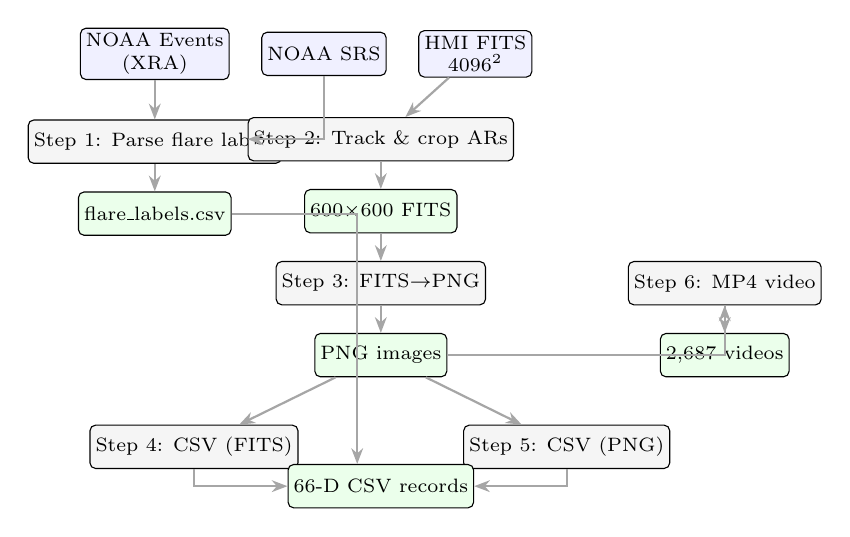
\begin{tikzpicture}[
  node distance=0.35cm and 0.4cm,
  box/.style={draw, rounded corners=2pt, align=center, font=\scriptsize,
              minimum height=0.55cm, inner sep=2pt, fill=gray!8},
  databox/.style={box, fill=blue!6},
  outbox/.style={box, fill=green!8, minimum width=1.6cm},
  arr/.style={-{Stealth[length=2mm]}, thick, gray!70}
]
  % Inputs
  \node[databox] (ev) {NOAA Events\\(XRA)};
  \node[databox, right=of ev] (srs) {NOAA SRS};
  \node[databox, right=of srs] (hmi) {HMI FITS\\4096$^2$};

  % Step 1
  \node[box, below=0.5cm of ev] (s1) {Step 1: Parse flare labels};
  \node[outbox, below=of s1] (lbl) {flare\_labels.csv};

  % Step 2
  \node[box, below=0.5cm of hmi, xshift=-1.2cm] (s2) {Step 2: Track \& crop ARs};
  \node[outbox, below=of s2] (fits) {600$\times$600 FITS};

  % Step 3
  \node[box, below=of fits] (s3) {Step 3: FITS$\to$PNG};
  \node[outbox, below=of s3] (png) {PNG images};

  % Steps 4-5
  \node[box, below left=0.6cm and 0.2cm of png] (s4) {Step 4: CSV (FITS)};
  \node[box, below right=0.6cm and 0.2cm of png] (s5) {Step 5: CSV (PNG)};
  \node[outbox, below=1.1cm of png] (csv) {66-D CSV records};

  % Step 6
  \node[box, right=1.8cm of s3] (s6) {Step 6: MP4 video};
  \node[outbox, below=of s6] (mp4) {2{,}687 videos};

  % Arrows
  \draw[arr] (ev) -- (s1);
  \draw[arr] (s1) -- (lbl);
  \draw[arr] (srs) |- (s2);
  \draw[arr] (hmi) -- (s2);
  \draw[arr] (s2) -- (fits);
  \draw[arr] (fits) -- (s3);
  \draw[arr] (s3) -- (png);
  \draw[arr] (png) -- (s4);
  \draw[arr] (png) -- (s5);
  \draw[arr] (s4) |- (csv);
  \draw[arr] (s5) |- (csv);
  \draw[arr] (lbl.east) -| ([xshift=-0.3cm]csv.north);
  \draw[arr] (png.east) -| (s6);
  \draw[arr] (s6) -- (mp4);
\end{tikzpicture}
\caption{End-to-end JW-FD construction pipeline. NOAA Events supply flare ground truth; SRS reports and HMI full-disk magnetograms define active-region crops. Steps~4 and~5 share the same 29-dimensional feature extractor and label-matching logic on FITS and PNG branches, respectively.}
\label{fig:pipeline}
\end{figure}


Table~\ref{tab:pipeline} summarizes inputs and outputs. Table~\ref{tab:config} lists key configurable parameters from \texttt{config.py}.

\begin{table}[t]
\caption{Pipeline step inputs and outputs.}
\label{tab:pipeline}
\centering
\scriptsize
\begin{tabular}{@{}clp{3.5cm}p{3.0cm}@{}}
\toprule
Step & Script & Input & Output \\
\midrule
1 & \texttt{step1\_extract\_flare\_labels} & NOAA Events \texttt{.txt} (XRA) & \texttt{flare\_labels.csv} \\
2 & \texttt{step2\_crop\_active\_regions} & SRS + HMI FITS (4096$^2$) & \texttt{fits\_600/\{AR\}/} \\
3 & \texttt{step3\_convert\_to\_png} & Step~2 FITS & \texttt{png\_600\_Th\{$B_{\mathrm{th}}$\}/} \\
4 & \texttt{step4\_generate\_dataset\_fits} & FITS + labels & \texttt{dataset\_fits\_*.csv} \\
5 & \texttt{step5\_generate\_dataset\_png} & PNG + labels & \texttt{dataset\_png\_*.csv} \\
6 & \texttt{step6\_make\_movie} & PNG sequences & \texttt{movies\_600\_Th\{$B_{\mathrm{th}}$\}/} \\
\bottomrule
\end{tabular}
\end{table}

\begin{table}[t]
\caption{Key pipeline configuration parameters.}
\label{tab:config}
\centering
\scriptsize
\begin{tabular}{@{}llp{4.2cm}@{}}
\toprule
Parameter & Default & Role \\
\midrule
\texttt{crop\_size} & 300 (600$^2$ output) & Half-width of AR crop \\
\texttt{mag\_threshold} & 200/500/1000~G & PNG saturation level \\
\texttt{prediction\_hours} & 1,3,6,12,24,48,72 & Label forecast horizons \\
\texttt{max\_longitude} & 60$^\circ$ & Disk-center limb filter \\
\texttt{centroid\_search\_size} & 80~px & Anchor refinement window \\
\texttt{centroid\_threshold} & 100~G & Strong-field mask for centroid \\
\texttt{max\_workers} & 64 & Multiprocessing pool size \\
\bottomrule
\end{tabular}
\end{table}

\subsection{Step 1: Flare label extraction}

NOAA daily Events files report XRA flare lines with begin, maximum, and end times and GOES class strings (e.g., M5.3). The parser reads the \texttt{:Date:} header, extracts XRA rows, and applies regular expressions for GOES classes matching C/M/X followed by a numeric sub-class. Records with missing peak time are discarded; missing begin or end times are replaced by the peak time. The associated AR must appear as a four-digit NOAA number. Timestamps are formatted as \texttt{YYYYMMDD\_HHMMSS}. Output columns are \texttt{AR\_Number}, \texttt{Begin\_Time}, \texttt{Max\_Time}, \texttt{End\_Time}, and \texttt{Flare\_Class}. Multiprocessing activates when more than 100 event files are present.

\subsection{Step 2: Active-region cropping and tracking}

SRS daily reports list NOAA AR numbers and heliographic locations. The parser converts compact location strings to signed latitude and longitude: north/south determine latitude sign; east is assigned negative longitude and west positive longitude in the internal Stonyhurst convention, consistent with HMI coordinate handling.

\textbf{Carrington anchor.} For each AR, an initial Carrington coordinate is obtained by transforming the SRS Stonyhurst position at the first available magnetogram epoch using \texttt{sunpy}. Because ARs traverse the disk as the Sun rotates, a fixed heliographic position is tracked through time by re-transforming the Carrington anchor to each observation epoch. Among subsampled daily FITS files, the frame with minimum absolute Stonyhurst longitude (nearest central meridian) is selected to reduce projection distortion before centroid refinement.

\textbf{Centroid correction.} Within an 80-pixel search window around the projected anchor, pixels with $|\mathrm{B}| > 100$~G define a mask; the center of mass yields a refined anchor. If the offset exceeds 150~pixels, the coarse anchor is retained.

\textbf{Parallel cropping.} For each full-disk FITS file, all ARs listed in that day's SRS are processed. The anchor is transformed to the observation epoch, converted to pixel coordinates, and cropped as a 600$\times$600 sub-array (300-pixel radius). ARs with $|\mathrm{longitude}| > 60^\circ$ are excluded; crop centers must lie sufficiently inside the 4096-pixel disk boundary.

\subsection{Step 3: FITS to PNG conversion}

Cropped FITS magnetograms are read as 32-bit arrays and left-right flipped (\texttt{fliplr}) so that display follows the north-up, east-left convention. Magnetic values are saturated and normalized:
\begin{equation}
B' = \mathrm{clip}(B,\,-B_{\mathrm{th}},\,B_{\mathrm{th}}), \quad
I = \frac{B' - \min(B')}{\max(B') - \min(B')} \times 255,
\label{eq:norm}
\end{equation}
where NaN pixels are replaced before clipping. Supported $B_{\mathrm{th}}$ values include 200, 500, and 1000~G; output directory names encode the chosen threshold.

\subsection{Steps 4--5: Feature extraction and CSV generation}

Two parallel branches generate CSV datasets from FITS (Step~4) and PNG (Step~5) inputs using the same 29-dimensional feature extractor and label-matching logic. PNG inputs are converted to grayscale when RGB. Features follow the methodology of Boucheron et al.,\cite{Boucheron2015} implemented in \texttt{feature\_extraction.py}:

\textbf{Gradient features} (7): Sobel operators convolved with the magnetogram yield gradient magnitude; mean, standard deviation, median, extrema, skewness, and kurtosis are computed over the magnitude map.

\textbf{Neutral-line features} (13): a 10$\times$10 uniform smoothing filter is applied; zero-level contours define neutral lines. Gradient-weighted neutral-line length, fragment count, and statistics of contour curvature and bending energy follow Ref.~\citenum{Boucheron2015}.

\textbf{Wavelet features} (5): a five-level Haar two-dimensional wavelet decomposition (\texttt{pywt.wavedec2}) yields sub-band energy sums L1--L5.

\textbf{Flux integrals} (4): total positive, negative, signed, and unsigned magnetic flux are computed by summing pixel values over positive and negative regions.

For PNG-derived features, pixel values are offset by 128 before computation (\texttt{extract\_all\_features}). Table~\ref{tab:features} lists all 29 feature names. Each image filename is parsed for AR identity and observation time; flare labels from Step~1 are matched under the rule in Sec.~\ref{sec:schema}.

\begin{table}[t]
\caption{Twenty-nine magnetic features extracted per snapshot (from \texttt{FEATURE\_NAMES}).}
\label{tab:features}
\centering
\scriptsize
\begin{tabular}{@{}ll@{}}
\toprule
Category & Feature names \\
\midrule
Gradient (7) & mean, std, median, min, max, skewness, kurtosis \\
Neutral line (13) & length; no.\ fragments; grad.-weighted length; \\
& curvature mean/std/median/min/max; \\
& bending energy mean/std/median/min/max \\
Wavelet (5) & Energy L1, L2, L3, L4, L5 \\
Flux (4) & positive, negative, signed, unsigned \\
\bottomrule
\end{tabular}
\end{table}

\subsection{Step 6: Evolution video synthesis}

For each AR directory, PNG frames are sorted chronologically, padded to dimensions divisible by 16, converted to RGB if grayscale, and encoded as H.264 MP4 at 60~fps. Each AR yields one \texttt{AR\{num\}\_evolution.mp4} file.

\subsection{Implementation notes}

Steps~1--6 use Python \texttt{multiprocessing.Pool} with configurable worker counts and batch preloading (\texttt{preload\_count}). Each step writes a dedicated log file under \texttt{logs/}. Failed file reads are recorded without halting the full run. Partial execution (\texttt{python run\_pipeline.py 4 5}) supports regenerating CSV branches after parameter changes.

\section{RECORD SCHEMA AND LABEL DESIGN}
\label{sec:schema}

Each CSV row describes one magnetogram snapshot. The 66-dimensional record comprises 29 magnetic features, 28 binary flare labels, 7 class-label strings, and 2 metadata fields (Table~\ref{tab:schema}).

\begin{table}[t]
\caption{66-dimensional CSV record structure.}
\label{tab:schema}
\centering
\small
\begin{tabular}{@{}clp{5.0cm}@{}}
\toprule
Block & Dim. & Content \\
\midrule
Magnetic features & 29 & Gradient, neutral line, wavelet, flux (Table~\ref{tab:features}) \\
Binary flare labels & 28 & 7 horizons $\times$ 4 thresholds \\
Class labels & 7 & Strongest GOES class per horizon \\
File metadata & 2 & \texttt{image\_filename}, \texttt{image\_path} \\
\midrule
Total & 66 & \\
\bottomrule
\end{tabular}
\end{table}

Prediction horizons are $h \in \{1,3,6,12,24,48,72\}$~hours. For each horizon~$h$ and threshold~$\tau \in \{\mathrm{C1.0,M1.0,M5.0,X1.0}\}$, the binary column \texttt{flare\_label\_\{$\tau$\}\_\{$h$hr\}} equals~1 if and only if there exists a flare event in the same AR whose begin time $\mathrm{Begin}$ satisfies
\begin{equation}
\mathrm{Begin} - h \;\le\; t \;<\; \mathrm{Begin}
\label{eq:window}
\end{equation}
and whose GOES class meets or exceeds~$\tau$ via the ordering C$<$M$<$X with numeric sub-class comparison; otherwise the label is~0. The column \texttt{flare\_class\_\{$h$hr\}} stores the strongest qualifying class, or \texttt{0} if none qualify.

% Pre-eruption label window: sample times (arrows) + positive window block
\begin{figure}[t]
\centering
\small
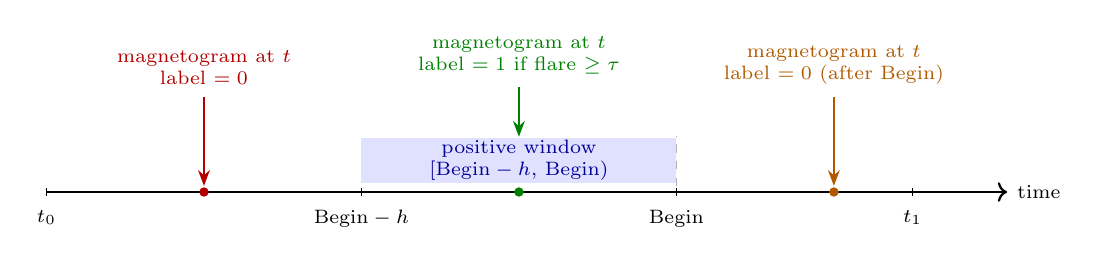
\begin{tikzpicture}[
  x=1.0cm, y=0.65cm,
  lbl/.style={font=\scriptsize},
  arr/.style={-{Stealth[length=2mm]}, semithick}
]
  % Time axis
  \draw[thick,->] (0,0) -- (12.2,0) node[right, lbl] {time};

  % Boundary ticks (below axis)
  \foreach \x/\t in {0/{$t_0$}, 4/{$\mathrm{Begin}-h$}, 8/{$\mathrm{Begin}$}, 11/{$t_1$}} {
    \draw (\x,0.07) -- (\x,-0.07);
    \node[lbl, below=3pt] at (\x,0) {\t};
  }

  % Begin boundary (open interval endpoint)
  \draw[dashed, gray!60] (8,0.12) -- (8,1.10);

  % Positive window block with label inside
  \fill[blue!12] (4,0.18) rectangle (8,1.05);
  \node[lbl, blue!60!black, align=center] at (6,0.62)
    {positive window\\$[\mathrm{Begin}-h,\,\mathrm{Begin})$};

  % Three example magnetogram times on the axis
  \fill[red!70!black] (2.0,0) circle (1.7pt);
  \fill[green!50!black] (6.0,0) circle (1.7pt);
  \fill[orange!70!black] (10.0,0) circle (1.7pt);

  % Arrows mark sample times; middle tip stops on the block top (not through the text)
  \draw[arr, red!70!black] (2.0,1.85) -- (2.0,0.12);
  \node[lbl, red!70!black, align=center, above=1pt] at (2.0,1.85)
    {magnetogram at $t$\\label $= 0$};

  \draw[arr, green!50!black] (6.0,2.05) -- (6.0,1.08);
  \node[lbl, green!50!black, align=center, above=1pt] at (6.0,2.05)
    {magnetogram at $t$\\label $= 1$ if flare $\geq\tau$};

  \draw[arr, orange!70!black] (10.0,1.85) -- (10.0,0.12);
  \node[lbl, orange!70!black, align=center, above=1pt] at (10.0,1.85)
    {magnetogram at $t$\\label $= 0$ (after $\mathrm{Begin}$)};
\end{tikzpicture}
\caption{Pre-eruption labeling window for horizon~$h$. A magnetogram observed at time~$t$ receives a positive binary label for threshold~$\tau$ only if $t \in [\mathrm{Begin}-h,\,\mathrm{Begin})$ and the matched GOES class meets or exceeds~$\tau$. Observations at or after $\mathrm{Begin}$ (dashed line) are excluded from the positive class.}
\label{fig:label_timeline}
\end{figure}


Figure~\ref{fig:label_timeline} illustrates the labeling window. For example, if $\mathrm{Begin = 12{:}00}$ UTC and $h = 24$~h, a magnetogram at 11:00 may receive a positive label for an impending M1.0 event, whereas a magnetogram at 12:00 or later is never positive for that event regardless of flare intensity---this excludes post-eruption frames from the positive class and enforces a forecasting semantics appropriate for operational lead-time studies.

When multiple flares fall within the same window for a given horizon, the strongest GOES class is retained. Threshold columns are derived from the stored class string: e.g., \texttt{flare\_label\_M1.0\_24hr}~=~1 if the matched class is M1.0 or stronger.

\section{MULTIMODAL SPATIOTEMPORAL ALIGNMENT}
\label{sec:alignment}

Ensuring consistency across FITS, PNG, CSV, and MP4 modalities is central to JW-FD's design.

\textbf{Temporal alignment.} All products share UTC timestamps parsed from HMI filenames (\texttt{YYYYMMDD\_HHMMSS}). Flare labels from NOAA Events are matched to magnetogram observation times through the pre-eruption window of Eq.~(\ref{eq:window}). MP4 videos preserve chronological frame order at fixed frame rate; each frame index maps one-to-one to a source PNG and thus to a CSV row.

\textbf{Spatial alignment.} FITS crops define the native pixel grid. PNG conversion applies only saturation, normalization, and a consistent left-right flip---no rescaling---so PNG pixels correspond one-to-one with FITS pixels. The 29-D feature vector is computed from the same array passed to each branch (FITS Gauss values or normalized PNG intensities). MP4 frames inherit the PNG spatial reference.

\textbf{Composite key.} The pair (\texttt{AR\_Number}, timestamp) uniquely identifies a snapshot across all modalities. CSV metadata columns \texttt{image\_filename} and \texttt{image\_path} provide human-readable pointers into the per-AR directory structure. This binding enables multimodal models to retrieve imagery, features, and labels for any indexed sample without external lookup tables.

\section{QUALITY ASSURANCE AND EVALUATION PROTOCOL}
\label{sec:qc}

\subsection{Automated quality control}

Quality gates are embedded at each pipeline stage. Step~1 discards events with invalid AR numbers, missing peak times, or unparseable GOES classes. Step~2 rejects crops whose centers fall outside the valid disk region or whose AR longitude exceeds the configured bound; subsampled anchor search limits compute cost while maintaining positional accuracy. Step~3 logs truncated FITS reads. Steps~4--5 skip empty or unreadable files and record per-file failures in step logs. NaN magnetic values are replaced during PNG normalization.

\subsection{Expert verification}

Following automated processing, solar-physics experts manually inspected approximately 5\% of randomly selected samples, verifying anchor placement, crop boundary completeness, and label alignment for M/X-class events. Identified bad frames---due to telescope gaps or processing edge cases---were excluded or reprocessed through parameter adjustment.

\subsection{AR-level data split}

JW-FD adopts an \textbf{8:1:1 random split at the AR level}: all snapshots belonging to one AR appear exclusively in the training, validation, or test partition. Consecutive HMI frames of the same AR exhibit strong temporal autocorrelation; assigning different timestamps of one AR to both training and test sets constitutes information leakage and inflates skill scores.\cite{Barnes2016,Leka2019} The AR-level protocol prevents this and yields sample counts approximately proportional to 8:1:1. The AR-to-partition assignment list is distributed with the dataset release.

Researchers should note that positive labels are rare for high thresholds (M5.0, X1.0) and long horizons, producing class imbalance. Metrics such as true skill statistic (TSS) or Brier score are recommended over raw accuracy.\cite{Bloomfield2012}

\subsection{Discussion and limitations}

JW-FD serves as infrastructure for both classical tabular ML on 29-D features and end-to-end vision or MLLM approaches on PNG/MP4 inputs.\cite{Shao2025jwflare} Dual FITS and PNG CSV branches support physics-faithful analysis (Gauss-scale features) and vision-ready workflows (normalized intensities) from a single pipeline run.

Current limitations include: (1)~LOS magnetograms only---vector magnetic field data (e.g., SHARP) are not yet integrated;\cite{Bobra2014} (2)~reliance on NOAA AR numbering and SRS daily positions, which may lag rapid flux emergence; (3)~disk-center bias from the $|\mathrm{longitude}| \le 60^\circ$ filter, excluding high-latitude and limb ARs; and (4)~12-minute HMI cadence, which may undersample fast-evolving pre-flare configurations. Planned extensions include SDO/AIA multi-wavelength channels, SHARP vector-field ingestion, and operational near-real-time pipeline hooks.

\section{CONCLUSIONS}
\label{sec:concl}

We presented JW-FD, a 14-year multimodal solar flare forecasting dataset constructed through a reproducible six-step pipeline from SDO/HMI magnetograms and NOAA flare reports. The release provides 1.75~million co-registered snapshots across FITS, PNG, CSV, and MP4 modalities, with 66-dimensional records linking 29 magnetic features to configurable pre-eruption labels over seven forecast horizons and four GOES thresholds. Multimodal spatiotemporal alignment is enforced through a composite AR-number and timestamp key. An AR-level 8:1:1 split establishes a leakage-free evaluation protocol for classical ML, deep vision models, and MLLMs.

Future work will integrate multi-wavelength SDO/AIA observations, extend temporal coverage through Solar Cycle~25, incorporate vector magnetogram parameters, and develop operational ingestion interfaces for near-real-time space-weather forecasting. The open-source pipeline (\texttt{https://github.com/Xiaoxuan-1/JW-FD}) enables the community to reproduce, extend, and benchmark flare-forecasting methods on a shared, long-horizon data foundation.

\acknowledgments
We thank the SDO/HMI team and NOAA Space Weather Prediction Center for providing open data products. This work was supported by the National Astronomical Observatories, Chinese Academy of Sciences.

\bibliography{references}
\bibliographystyle{spiebib}

\end{document}
